\documentclass[12pt,oneside,a4paper]{article} % for sharing
\usepackage{apacite}
\usepackage{appendix}
\usepackage{amsmath}
\usepackage{amsthm}
\usepackage{multirow}
\usepackage{amssymb} % for approx greater than
\usepackage{caption}
\usepackage{placeins} % for \FloatBarrier
\usepackage{graphicx}
\usepackage{subcaption}
\usepackage{longtable}
\usepackage{setspace}
\usepackage{booktabs}
\usepackage{tabularx}
\usepackage{xcolor,colortbl}
\usepackage{chngpage}
\usepackage{natbib}
\bibpunct{(}{)}{,}{a}{}{;} 
\usepackage{url}
\usepackage{nth}
\usepackage{authblk}
\usepackage[most]{tcolorbox}
\usepackage[normalem]{ulem}
\usepackage{amsfonts}



% columns for longtable
\newcolumntype{C}[1]{>{\centering\let\newline\\\arraybackslash\hspace{0pt}}m{#1}}
\newcolumntype{L}[1]{>{\raggedright\let\newline\\\arraybackslash\hspace{0pt}}m{#1}}
\usepackage{arydshln} % Dashed lines in matrices

\usepackage[margin=1in]{geometry}
%\doublespacing % for review

% line numbers to make review easier
%\usepackage{lineno}
%\linenumbers

%\usepackage{soul}% for \st{}

%%%%%%%%%%%%%%%%%%%%%%%%%%%%%%%%%%%%%%%%%%%%%%%%%%%%%%%%%%%%%%%%%%%%%%%%%%%%%%
% for section 4 math environments
\theoremstyle{definition}
\newtheorem{definition}{Definition}[section]
\newtheorem{theorem}{Theorem}[section]
\newtheorem{proposition}{Proposition}[section]
\newtheorem{corollary}{Corollary}[proposition]
\newtheorem{remark}{Remark}[section]

%%%%%%%%%%%%%%%%%%%%%%%%%%%%%%%%%%%%%%%%%%%%%%%%%%%%%%%%%%%%%%%%%%%%%%%%%%%%%%

\newcommand\ackn[1]{%
  \begingroup
  \renewcommand\thefootnote{}\footnote{#1}%
  \addtocounter{footnote}{-1}%
  \endgroup
}

% Affiliations in small font size
\renewcommand\Affilfont{\small}

\defcitealias{HMD}{HMD 2016}

% junk for longtable caption
\AtBeginEnvironment{longtable}{\linespread{1}\selectfont}
\setlength{\LTcapwidth}{\linewidth}

% sort van Raalte properly
% #1: sorting key, #2: prefix for citation, #3: prefix for bibliography
\DeclareRobustCommand{\VAN}[3]{#2} % set up for citation

%%%%%%%%%%%%%%%%%%%%%%%%%%%%%%%
\begin{document}


\title{Area level inequalities in variation in age at death: have the between-group and within-group contributions changed over time?}
%\author{author(s) redacted}
\author[1]{Rosie Seaman\thanks{seaman@demogr.mpg.de}}
\author[2]{Hal Caswell}
\author[1]{Tim Riffe}

\affil[1]{Max Planck Institute for Demographic Research, Rostock, Germany}
\affil[2]{University of Amsterdam}

\maketitle

\begin{abstract}
Mortality inequality implies a double burden: The most deprived socioeconomic
groups experience the lowest average age of death and the highest variation in age at death. No study has identified how variation in age of death is patterned by area-level socioeconomic deprivation despite the established literature demonstrating that area-level effects are an important part of the explanation for inequalities in risk of death. Two underlying processes drive variation in age at death: individual stochasticity (within-group inequality) and heterogeneity (between-group inequality). Limited research has evaluated how these two components have changed over time. We address these research gaps by using population and mortality data for the entire population of Scotland stratified by a validated measure of area-level deprivation that covers the time period 1981-2011.
\end{abstract}

\section{Background}
The association between socioeconomic inequality and mortality is traditionally
evidenced by life expectancy comparisons. The most deprived populations
experience the lowest average age of death, and the least deprived populations
experience the highest. Studies have further demonstrated that the most deprived
populations also demonstrate the highest level of variation in age at death when
measuring socioeconomic inequality by income, education, or occupation
\citep{bronnum2007increasing, vaupel2011life, van2014lifespan,
sasson2016trends}. No study to our knowledge has identified how variation in age
of death is patterned when measuring socioeconomic inequality by area-level deprivation even though it has long been established that area of residence is an important part of the explanation for socioeconomic differences in mortality outcomes (Carstairs and Morris 1989; Macintyre, Ellaway and Cummins 2002). Area-level measures aim to capture the theoretical notion of relative deprivation rather than absolute poverty. Relative deprivation is the idea that not having enough material cultural or social resources to participate in the accepted way of life in the given society is as important for health as the absolute minimum requirements for survival (Carstairs and Morris 1989; Kearns, Gibb and Mackay 2000; Townsend 1987).
 
Two underlying processes drive variance in age at death: individual stochasticity (within group inequality) and heterogeneity (between group inequality). Within group inequality arises from variance due to random demographic processes. For example, a life table assumes that every individual is subject to the exact same mortality rates stipulated in that life table and any variance in age of death can be interpreted as individual stochasticity. Between group inequality can arise if individuals at the same age are subject to different mortality rates that may be due to unobserved social, economic or environmental contexts (Hartemink, Missov and Caswell 2017). 

One existing study of 11 European countries found that the differences between educational groups accounted for between 1.2\% and 10.9\% of total variance in age at death (van Raalte et al. 2012). This study used aggregated data for the years  1990 to 2000 meaning that any changes in the components of total inequality could not be assessed. Education may also be a problematic socioeconomic measure for studying changes in components over time because of compositional changes.  In addition, stratifying data by education meant that data for ages $<$35 were truncated out of the analysis. 
 
We build on the important findings of this study by evaluating how the within group and between group components of total variance in age at death are patterned by sex, area-level deprivation and over time. We use decennial Census population estimates and mortality data stratified into population weighted quintiles according to a validated area-level measure of relative deprivation. The data  include the whole population of Scotland and cover the time period between 1981 and 2011. Using population weighted quintiles according to an area-level measure of deprivation has two advantages. Firstly, it is applicable to the entire population meaning that age truncation is not necessary. Secondly, it is a relative measure of deprivation meaning that there is always a notional 20\% most deprived compared to a notional 20\% least deprived even though absolute levels of deprivation may have changed over time. 


\section{Data and methods}

\subsection{Area level deprivation}
Census population estimates and mortality  data\footnote{All years of mortality data used were 1980-1982, 1990-1991, 2000-2002 and 2010-2012 to increase the number of events. 1990-1991 only due to geographical boundary changes occurring in 1990. Corresponding Census population estimates multiplied accordingly.} by single year of age and sex for each part-postcode (zip code) sector in Scotland  were obtained via a commissioned request to National Records of Scotland. There are around 1,012 part-postcode sectors in Scotland at each Census year each with an average population size of 5,000 individuals.
 
Population weighted quintiles (20\% of the population) were created by aggregating the 1,012 part-postcode sectors according to Carstairs score of deprivation. The Carstairs score is a z-score for each part-postcode sector is derived from four individual level Census variables: overcrowding, male unemployment, low social class and no car ownership. The Carstairs Score (z-score) reflects the material resources which provide the means to access the goods, services, amenities and physical environment which are seen as expected in society (Carstairs and Morris 1990). This means the Carstairs score is a method of capturing relative deprivation at the contextual level.

These data were utilized to construct complete lifetables for each deprivation quintile, at each Census year, for males and females seperately (40 lifetables in total). The Human Mortality database protocol was used to extrapolate age specific mortality rates for ages 85 to 110+ (Wilmoth et al. 2007). From the complete lifetables we compute life expectancy and use the standard deviation, a standard statistical measurement of the variability applied to the distribution of age at death (van Raalte and Caswell 2013). Details of the within group and between group component calculations are given in the following subsection.


\subsection{Variance decomposition}

 The index $k$ refers to each deprivation quintile. Given $p_x = 1- q_x$ for a quintile, calculate:
\begin{equation}
\mathbf{U}_k = 
\begin{bmatrix}
    0     & \hdots  & \hdots &  \hdots  & 0 \\
    p_{1} &   &    &    &  \vdots \\
    0 & \ddots &   &   & \vdots \\
    \vdots & & \ddots & & 0\\
   0 &  \hdots & 0 & p_{\omega-1}  & p_{\omega}
\end{bmatrix}
\end{equation}
Then calculate the conditional remaining survivorship as
\begin{equation}
\mathbf{N}_k = (\mathbf{I} - \mathbf{U}_k )^{-1} \quad .
\end{equation}
$\mathbf{N}_k$ ends up being 0s in the upper triangle, and conditional remaining
survivorship in columns descending from the subdiagonal. The first moment is the
same as remaining life expectancy, and can be calculated as:
\begin{equation}
\eta^{(k)}_1 = (1^T \mathbf{N}_k)^T
\end{equation}
The second moment is defined as:
\begin{equation}
\eta^{(k)}_2 = \left[ 1^T \mathbf{N}_k (2\mathbf{N}_k - \mathbf{I})\right]^T
\end{equation}
These can be used together to calculate the variance of remaining lifespan:
\begin{equation}
\label{eq:var}
V(\eta^{(k)}) = \eta^{(k)}_2 - \left[\eta^{(k)}_1 \circ \eta^{(k)}_1 \right]
\end{equation}
Thus far everything has been denoted with respect to the $k^{th}$ quintile.
These may aggregate to a total lifetable for the entire population according to some mixing distribution,
$\pi$.
The most natural mixture is to to give age-specific weights according to
observed relative population counts in each subpopulation, $\pi(a,k)$. Other
mixtures may be based on an age-pattern to $\pi$ based on the stationary
population produced by each quintile's lifetable. By this method, lower
mortality lifetables result in greater relative weight in older ages. In this
case, weight is assigned only to the lifetable radix. In our case, the subpopulations are aggregated into
deprivation quantiles and they end up being of approximately equal size and the
uniform radix mixing distribution is not acceptable. In alternative cases it may be more appropriate to assign weights relative to the total population size of subpopulation, or simply
giving uniform weights.

Given $\pi(a,k)$ we can decompose the variance of the total
aggregation of subpopulations due to \eqref{eq:var} into variance due to
stochasticity within subpopulations and variance due to differences between
populations in the lifespan distribution. These two variance components sum to
\eqref{eq:var} when the same age vector $\pi^{(k)}$, is used to blend
lifetables for \eqref{eq:var} and in the following equations:
\begin{align}
V_{within} &= \mathbb{E}_\pi \left( V(\eta_1^{(k)})\right)\\
 &= \sum_{k=1}^N \pi_k V(\eta_1^{(k)})
\intertext{and}
V_{between} &= V_\pi \left( V(\eta_1^{(k)})\right)\\
 &= \sum_{k=1}^N \pi_k \circ \eta_1^{(k)} \circ \eta_1^{(k)} -
 \left[ \sum_{k=1}^N \pi_k \circ \eta_1^{(k)} \right] \circ \left[ \sum_{k=1}^N \pi_k
 \circ \eta_1^{(k)} \right]
\end{align}




\section{Preliminary results}

Table 1 and Table 2 show the life expectancy and variation in age at death for males and females in each deprivation quintile at each Census year. The same tables reporting life expectancy and variation in age at death conditional upon survival to age 35 are included in the appendices.  

% Table generated by Excel2LaTeX from sheet 'Sheet1'
\begin{table}[htbp]
  \centering
  \caption{Life expectancy and standard deviation for males, age 0.}
    \begin{tabular}{lrrrrrrrr}
          & \multicolumn{2}{c}{1981} & \multicolumn{2}{c}{1991} & \multicolumn{2}{c}{2001} & \multicolumn{2}{c}{2011} \\
    \midrule
    quintile & \multicolumn{1}{c}{ex} & \multicolumn{1}{c}{sd} & \multicolumn{1}{c}{ex} & \multicolumn{1}{c}{sd} & \multicolumn{1}{c}{ex} & \multicolumn{1}{c}{sd} & \multicolumn{1}{c}{ex} & \multicolumn{1}{c}{sd} \\
    \midrule
    1 (least dep.) & 71.6  & 15.4  & 74.5  & 14.4  & 77.6  & 13.7  & 80.2  & 13.6 \\
    2     & 69.9  & 16.1  & 72.9  & 14.9  & 75.3  & 15.1  & 78.5  & 14.6 \\
    3     & 69.1  & 16.2  & 72.1  & 15.4  & 73.9  & 15.4  & 77.0  & 15.1 \\
    4     & 68.2  & 16.2  & 70.4  & 16.1  & 72.2  & 16.1  & 75.3  & 15.6 \\
    5 (most dep.) & 66.4  & 16.4  & 68.3  & 16.5  & 69.0  & 17.2  & 72.4  & 16.5 \\
    Total pop. & 69.0  & 16.1  & 71.6  & 15.6  & 73.5  & 15.8  & 76.7  & 15.4 \\
    \bottomrule
    \end{tabular}%
  \label{tab:addlabel}%
\end{table}%


% Table generated by Excel2LaTeX from sheet 'Sheet1'
\begin{table}[htbp]
  \centering
  \caption{Life expectancy and standard deviation for females, age 0.}
    \begin{tabular}{lrrrrrrrr}
          & \multicolumn{2}{c}{1981} & \multicolumn{2}{c}{1991} & \multicolumn{2}{c}{2001} & \multicolumn{2}{c}{2011} \\
    \midrule
    quintile & \multicolumn{1}{c}{ex} & \multicolumn{1}{c}{sd} & \multicolumn{1}{c}{ex} & \multicolumn{1}{c}{sd} & \multicolumn{1}{c}{ex} & \multicolumn{1}{c}{sd} & \multicolumn{1}{c}{ex} & \multicolumn{1}{c}{sd} \\
    \midrule
    1 (least dep.) & 77.1  & 14.9  & 79.1  & 14.1  & 81.3  & 13.0  & 83.4  & 12.8 \\
    2     & 75.8  & 15.3  & 78.6  & 13.9  & 80.4  & 13.6  & 82.1  & 13.5 \\
    3     & 75.1  & 15.6  & 77.7  & 14.7  & 78.9  & 14.5  & 80.9  & 13.9 \\
    4     & 74.4  & 15.7  & 76.6  & 14.8  & 78.1  & 14.6  & 80.0  & 14.0 \\
    5 (most dep.) & 72.8  & 16.3  & 74.9  & 15.9  & 76.3  & 15.7  & 77.9  & 15.1 \\
    Total pop. & 75.0  & 15.6  & 77.3  & 14.8  & 78.9  & 14.4  & 80.9  & 14.0 \\
    \bottomrule
    \end{tabular}%
  \label{tab:addlabel}%
\end{table}%

The most deprived experience the lowest average life expectancy and the highest variation in age at death at each year. For males there was an increase in variation in age at death between 1991 and 2001. Although there was some improvement between 2001 and 2011 variation in age at death was very similar to the level experienced by males 30 years earlier. Females from the most deprived quintile have experienced decreasing variation in age at death but the decrease was far greater for the least deprived. The change in standard deviation over time, across all ages is visualised in Figure 1.

Figure 2 shows the proportion of the total difference in variation in age at death that is due to differences between area level deprivation. For males and females the proportion of variation explained by between group inequality has increased over time. The increase in this component was greater in magnitude for males than for females.

\begin{figure*}[t!]
    \centering
      \caption{Standard deviation of remaining lifespan by age, Census years
      1981 until 2011.}
    \begin{subfigure}[t]{0.5\textwidth}
        \centering
        \caption{Males}
        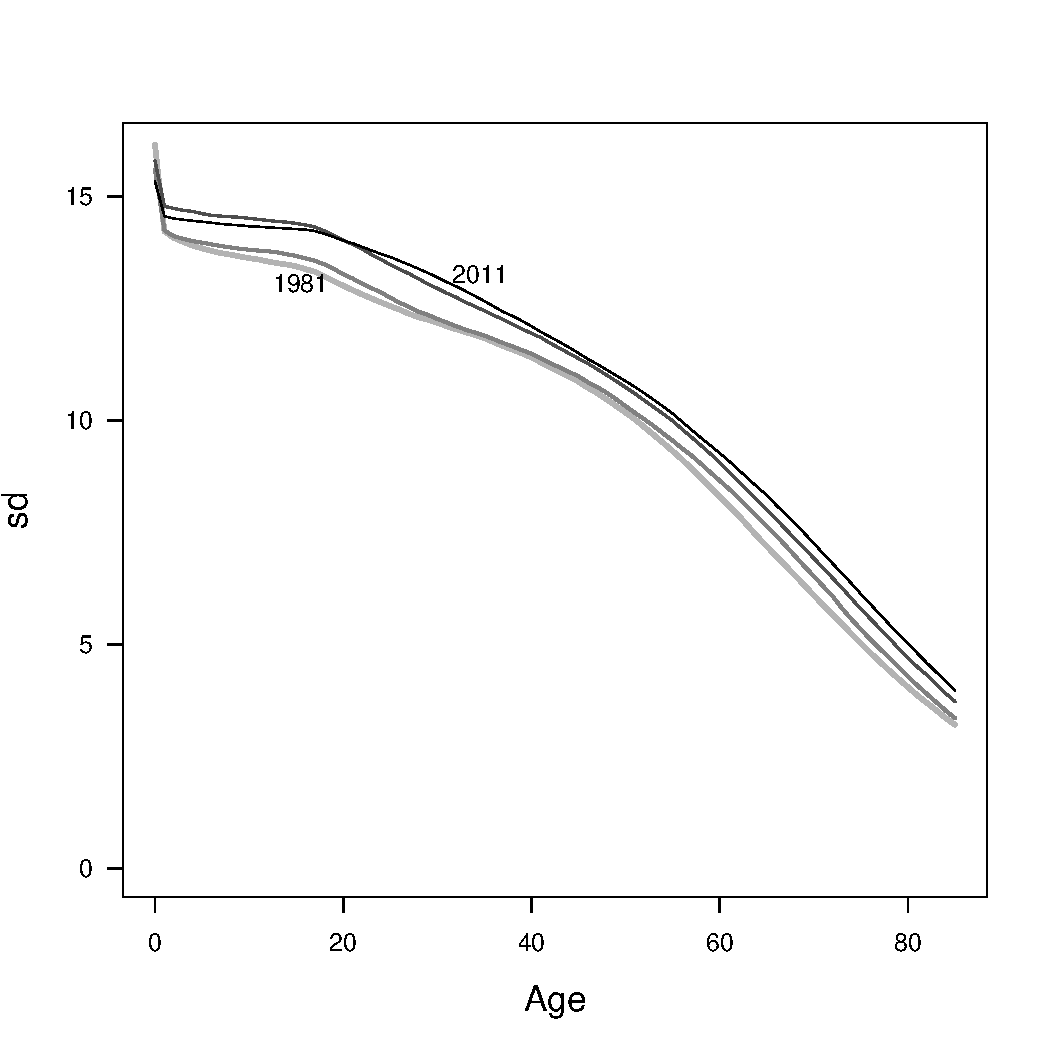
\includegraphics[width=\textwidth]{Figures/TotalsdMales.pdf}
    \end{subfigure}%
    ~ 
    \begin{subfigure}[t]{0.5\textwidth}
        \centering
        \caption{Females}
        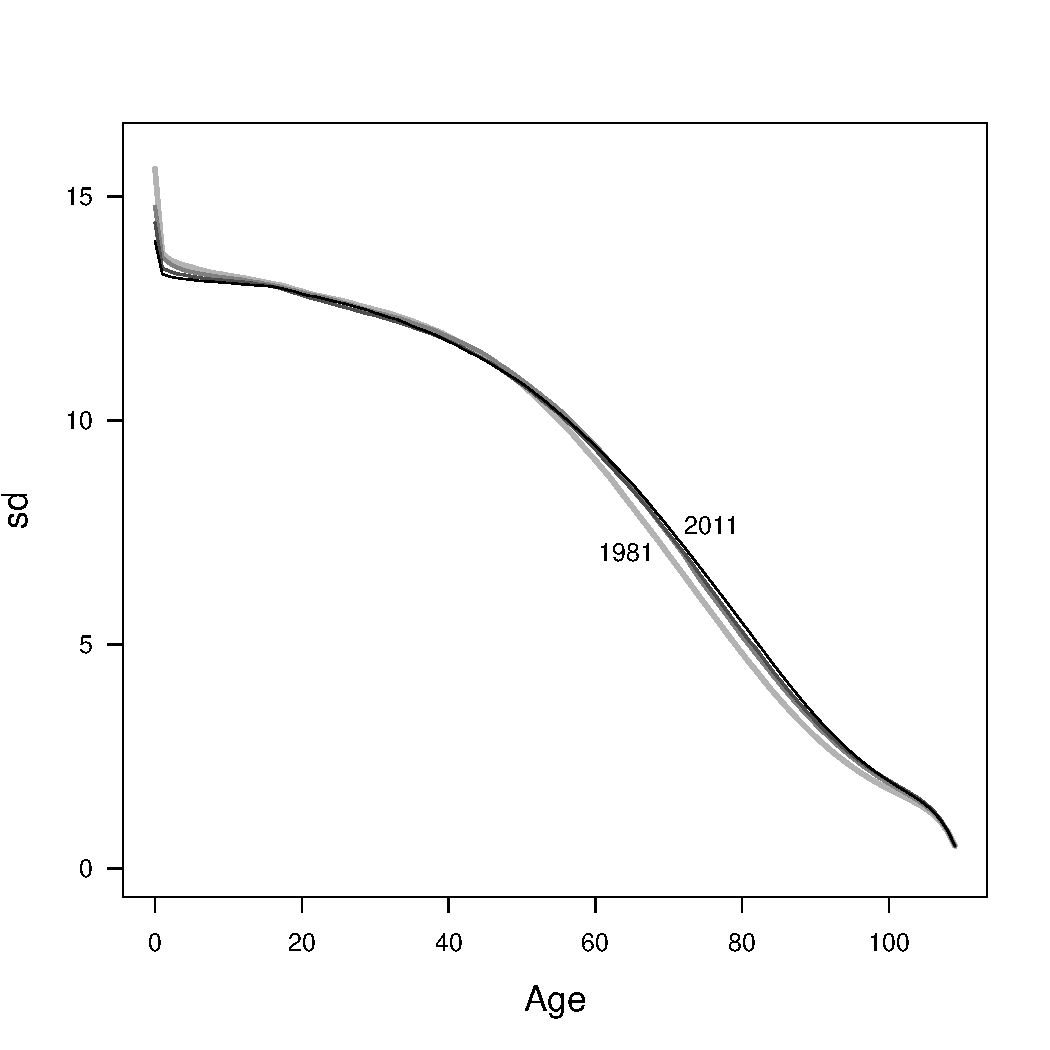
\includegraphics[width=\textwidth]{Figures/TotalsdFemales.pdf}
    \end{subfigure}
\end{figure*}

\begin{figure*}[t!]
    \centering
      \caption{Proportion of variance due to differences between deprivation
      quintiles by age, Census years 1981 until 2011.}
    \begin{subfigure}[t]{0.5\textwidth}
        \centering
        \caption{Males}
        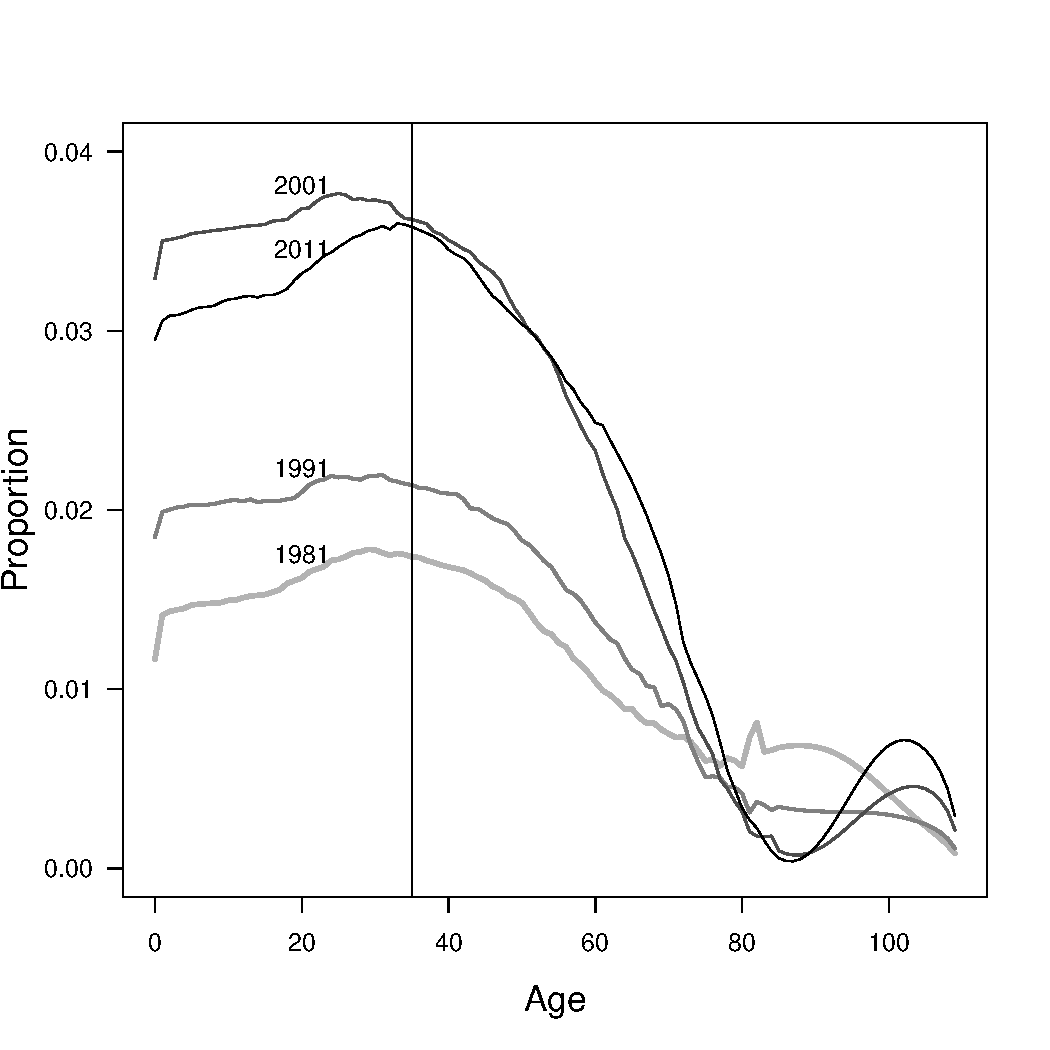
\includegraphics[width=\textwidth]{Figures/BetweenPropMales.pdf}
    \end{subfigure}%
    ~ 
    \begin{subfigure}[t]{0.5\textwidth}
        \centering
        \caption{Females}
        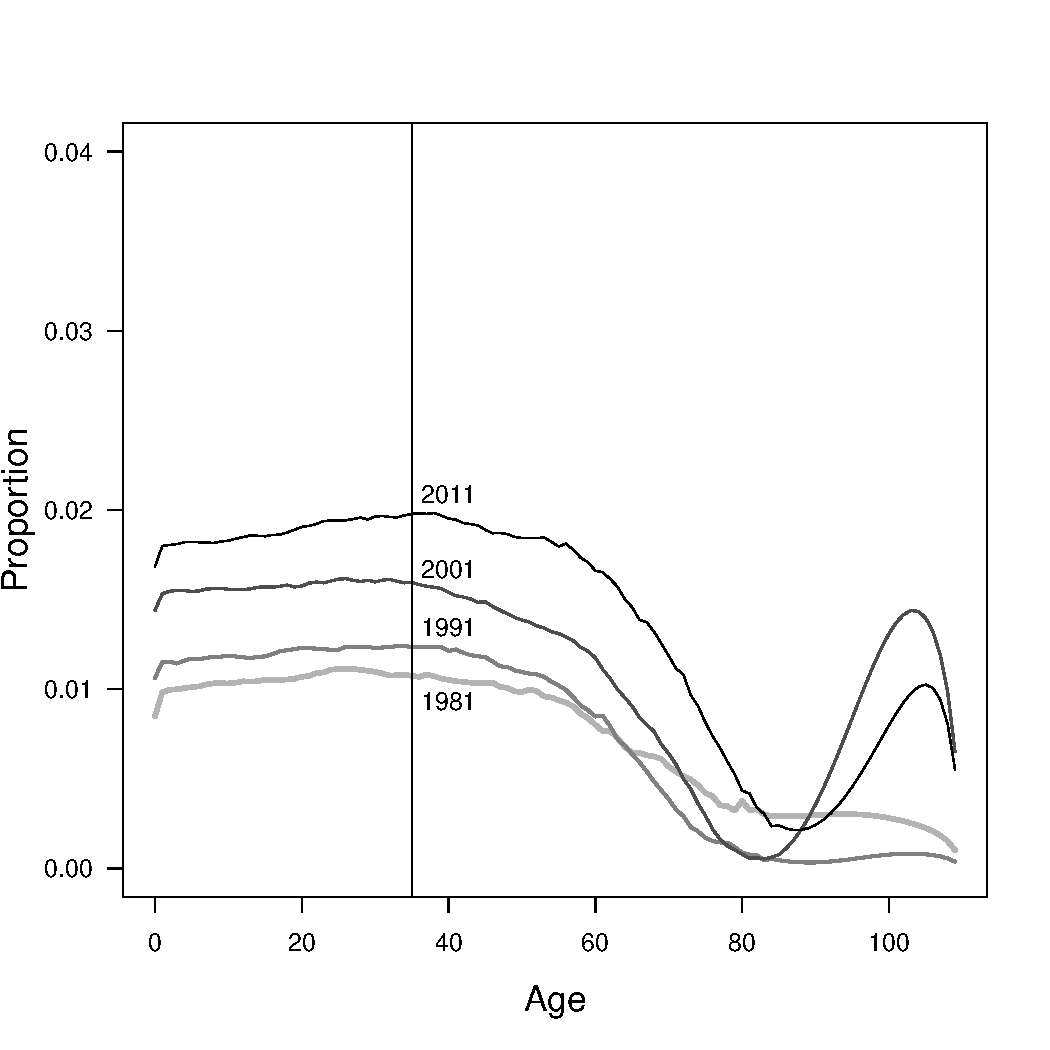
\includegraphics[width=\textwidth]{Figures/BetweenPropFemales.pdf}
    \end{subfigure}
\end{figure*}

\subsection{Sensitivity analysis}
We tested the sensitivity of our results to the size of deprivation group by replicating the analysis using deciles of deprivation, each representing 10\% of the population. The conclusions were the same for males and for females. However, the increase in the between group component over time was greater in magnitude when using deciles. We chose to report results for quintiles of deprivation as they are the preferred analytical grouping for routine reporting of health measures in Scotland (NHS: Public Health and Intelligence. 2017).

\section{Discussion and conclusion}

\subsection{Summary of main findings}
Deprivation differences in age at death were evident at all Census years when measuring socioeconomic inequality by area-level. Those living in the most deprived areas can expect to live the shortest lives and experience the greatest variation in age at death: a double burden of mortality inequality. The difference between deprivation groups was larger for males than for females. Males from the most deprived quintile experienced increasing variation in age at death between 1991 and 2001 so that the level of variation in 2011 was the same as that experienced 30 years earlier. The between group component of inequality also increased over the time period.

\subsection{Strengths and limitations}
The data used for this study includes the most robust population estimates and mortality data for the entire population of Scotland. Using a validated area-level measure of socioeconomic inequality meant that complete lifetables could be constructed and no ages were truncated from the analysis. However, it is important to acknowledge the reasons why studies interested in the social distribution mechanisms of adult mortality may consider restricting analysis to older ages. Smits and Monden (2009) suggest only looking at ages 15+ because these are the ages where 80\% of deaths in developed countries now occur. Looking only at adult mortality may better reflect the causes of death driving mortality change in more recent time periods: infectious disease and effective medical intervention historically reduced infant and childhood deaths rapidly but reductions in adult mortality are influenced by more complex mechanisms that change slowly (Smits and Monden 2009; Vallin and Meslé 2004). Our results indicate that the age at which the difference in variation in age at death is greatest is around 35 years old. This provides some reassurance for studies that are forced to truncate out younger age groups: the peak of variation in age at death (at least in developed countries) is likely to be captured. 

We recognize that our results are vulnerable to the ecological fallacy : it is possible that the association found at the area-level may differ from the association found at the individual (Diez 2002). The consistency of our findings with the existing literature on socioeconomic inequalities in variation in age at death (Brønnum-Hansen 2017; van Raalte et al. 2014) indicates that the findings by area-level deprivation are not an artefact. This does not mean that area-level measures and individual level measures are substitutes for one another. Area-level measures ‘capture characteristics of populations’ and individual level measures ‘capture characteristics of individuals’ (Leyland et al. 2007). An example helps to illustrate the contentions. GPs aiming to reduce inequalities between individuals by providing preventative screening programmes may rely on area-level indicators to target those who are most deprived but may target an individual in a deprived area who is actually well-off. So relying on an area-level measure to reduce health inequalities between individuals can be problematic if there is an assumption that the underlying characteristics of the population are socially homogenous (Fischbacher 2014). We acknowledge that deprived individuals do not exclusively reside in deprived areas and affluent individuals do not exclusively reside in affluent areas (Leyland et al. 2007).

The Carstairs score has been the focus of further criticisms. For example, the meaning of car ownership is fundamentally different for individuals in rural contexts compared to urban contexts. It is also acknowledged that overcrowding may occur out of choice and for cultural reasons rather than simply being a marker of deprivation (Fischbacher 2014). Therefore it has been suggested that the Carstairs score may be an out of date measure of socioeconomic deprivation (Schofield et al. 2016; Tunstall et al. 2011) because the relevance of the variables used for capturing the meaning of deprivation varies across contexts and over time (Norman 2010). In response, it was demonstrated that the scores for each postcode sector at each Census year are highly correlated despite changes to the formal definitions of the variables. This is interpreted as evidence that the underlying information the variables aim to capture is similar or that deprivation has remained stable over time (Leyland et al. 2007).

\section{Conclusion}
Area-level measures of deprivation are an invaluable tool for population health research. Perhaps more importantly, they have pragmatic advantages for governments seeking to identify how resources should be distributed across societies and are actively used by policies which intervene on neighborhoods or communities rather than individuals (Allik et al. 2016; Diez Roux 2001; Robert 1999; The Scottish Government and National Statistics 2012). For these reasons, it is important that more countries evaluate inequalities in variation in age at death by an area-level measure of socioeconomic inequality. This will help to identify if increasing contributions from between group inequality to total variation in age at death is a finding that is dependent upon, and thus amenable to, country specific contexts.  


\bibliographystyle{plainnat}
\bibliography{references}


\section{Appendices}
% Table generated by Excel2LaTeX from sheet 'Sheet1'
\begin{table}[htbp]
  \centering
  \caption{Life expectancy and standard deviation for males, age 35.}
    \begin{tabular}{lrrrrrrrr}
          & \multicolumn{2}{c}{1981} & \multicolumn{2}{c}{1991} & \multicolumn{2}{c}{2001} & \multicolumn{2}{c}{2011} \\
    \midrule
    quintile & \multicolumn{1}{c}{ex} & \multicolumn{1}{c}{sd} & \multicolumn{1}{c}{ex} & \multicolumn{1}{c}{sd} & \multicolumn{1}{c}{ex} & \multicolumn{1}{c}{sd} & \multicolumn{1}{c}{ex} & \multicolumn{1}{c}{sd} \\
    \midrule
    1 (least dep.) & 38.4  & 11.4  & 40.9  & 11.2  & 43.7  & 11.3  & 46.3  & 11.1 \\
    2     & 37.1  & 11.6  & 39.5  & 11.6  & 41.9  & 11.8  & 44.7  & 12.0 \\
    3     & 36.4  & 11.8  & 38.8  & 11.8  & 40.5  & 12.2  & 43.4  & 12.4 \\
    4     & 35.5  & 11.8  & 37.6  & 11.9  & 39.1  & 12.5  & 41.7  & 13.0 \\
    5 (most dep.) & 33.8  & 12.1  & 35.8  & 12.3  & 36.6  & 13.2  & 39.2  & 13.5 \\
    Total pop. & 36.2  & 11.8  & 38.5  & 11.8  & 40.3  & 12.4  & 43.1  & 12.6 \\
    \bottomrule
    \end{tabular}%
  \label{tab:addlabel}%
\end{table}%


% Table generated by Excel2LaTeX from sheet 'Sheet1'
\begin{table}[htbp]
  \centering
  \caption{Life expectancy and standard deviation for females, age 35.}
    \begin{tabular}{lrrrrrrrr}
          & \multicolumn{2}{c}{1981} & \multicolumn{2}{c}{1991} & \multicolumn{2}{c}{2001} & \multicolumn{2}{c}{2011} \\
    \midrule
    quintile & \multicolumn{1}{c}{ex} & \multicolumn{1}{c}{sd} & \multicolumn{1}{c}{ex} & \multicolumn{1}{c}{sd} & \multicolumn{1}{c}{ex} & \multicolumn{1}{c}{sd} & \multicolumn{1}{c}{ex} & \multicolumn{1}{c}{sd} \\
    \midrule
    1 (least dep.) & 43.4  & 11.7  & 45.1  & 11.5  & 47.0  & 11.1  & 49.0  & 49.0 \\
    2     & 42.2  & 12.0  & 44.4  & 11.7  & 46.1  & 11.5  & 47.9  & 47.9 \\
    3     & 41.6  & 12.2  & 43.8  & 12.1  & 45.0  & 12.0  & 46.7  & 46.7 \\
    4     & 41.0  & 12.1  & 42.7  & 12.3  & 44.1  & 12.2  & 45.7  & 45.7 \\
    5 (most dep.) & 39.6  & 12.7  & 41.4  & 12.8  & 42.6  & 13.1  & 43.9  & 43.9 \\
    Total pop. & 41.5  & 12.2  & 43.4  & 12.2  & 44.9  & 12.1  & 46.7  & 46.7 \\
    \bottomrule
    \end{tabular}%
  \label{tab:addlabel}%
\end{table}%


\end{document}